Two post-primary equal-call audits test different ways of exposing timing information on separate frozen inventories (Figure~\ref{fig:submission-critical-effects}). Convention-told effects are model-conditional (Qwen -5.0, GLM +10.0, DeepSeek +7.5, MiniMax +25.0 pp), whereas Decision-visible yields positive changed-winner PairAcc effects for all four models (Qwen +25.0, GLM +53.1, DeepSeek +43.8, MiniMax +34.4 pp). The inventories are not pooled; Convention-told and decision-block runs contain 1 and 0 incomplete ITT rows, respectively.

\begin{figure}[t]
\centering
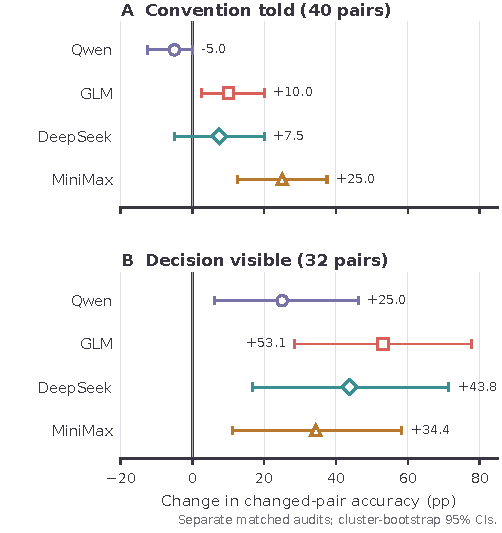
\includegraphics[width=0.97\columnwidth]{Figures/fig_submission_critical_pairacc_effects.pdf}
\caption{Post-primary equal-call contrasts on separate, unpooled inventories. A: natural-language Convention-told (40 changed pairs). B: complete Decision-visible block (32 actionable changed pairs). Bars are pair-cluster-resampling 95\% CIs over the tested authored clusters.}
\label{fig:submission-critical-effects}
\end{figure}
